\documentclass[c]{beamer}

\usetheme{Berlin}

%%% Работа с русским языком
\usepackage{cmap}					% поиск в PDF
\usepackage{mathtext} 				% русские буквы в формулах
\usepackage[T2A]{fontenc}			% кодировка
\usepackage[utf8]{inputenc}			% кодировка исходного текста
\usepackage[ukrainian,english,russian]{babel}	% локализация и переносы

%% Beamer по-русски
\newtheorem{rtheorem}{Теорема}
\newtheorem{rproof}{Доказательство}
\newtheorem{rexample}{Пример}

%%% Дополнительная работа с математикой
\usepackage{amsmath,amsfonts,amssymb,amsthm,mathtools} % AMS
\usepackage{icomma} % "Умная" запятая: $0,2$ --- число, $0, 2$ --- перечисление

%% Номера формул
%\mathtoolsset{showonlyrefs=true} % Показывать номера только у тех формул, на которые есть \eqref{} в тексте.
%\usepackage{leqno} % Нумерация формул слева

%% Свои команды
\DeclareMathOperator{\sgn}{\mathop{sgn}}

%% Перенос знаков в формулах (по Львовскому)
\newcommand*{\hm}[1]{#1\nobreak\discretionary{}
{\hbox{$\mathsurround=0pt #1$}}{}}

%%% Работа с картинками
\usepackage{graphicx}  % Для вставки рисунков
\graphicspath{{Mal/}}  % папки с картинками
\setlength\fboxsep{3pt} % Отступ рамки \fbox{} от рисунка
\setlength\fboxrule{1pt} % Толщина линий рамки \fbox{}
\usepackage{wrapfig} % Обтекание рисунков текстом

%%% Работа с таблицами
\usepackage{array,tabularx,tabulary,booktabs} % Дополнительная работа с таблицами
\usepackage{longtable}  % Длинные таблицы
\usepackage{multirow} % Слияние строк в таблице

%%% Программирование
\usepackage{etoolbox} % логические операторы

%%% Другие пакеты
\usepackage{lastpage} % Узнать, сколько всего страниц в документе.
\usepackage{soul} % Модификаторы начертания
\usepackage{csquotes} % Еще инструменты для ссылок
%\usepackage[style=authoryear,maxcitenames=2,backend=biber,sorting=nty]{biblatex}
\usepackage{multicol} % Несколько колонок

%%% Картинки
\usepackage{tikz} % Работа с графикой
\usepackage{pgfplots}
\usepackage{pgfplotstable}

\setbeamertemplate{footline}[frame number]

\title{Дипломна робота}
\subtitle{Розробка методів представлення візуальної інформації за допомогою методів самонавчання та contrastive learning}
\author{Виконав: студент групи КН-Н119, \\ Гончаров В. А. \\
Керівник дипломної роботи: ст. викладач каф. КМАД \\ Колбасін В. О.}
\date{Харків 2021}
\institute[НТУ <<ХПІ>>]{
 Міністерство Освіти і Науки України \\
Національний технічний університет <<Харківський політехнічний інститут>> \\
Факультет: Комп’ютерних наук та програмної інженерії \\
Кафедра: Комп’ютерної математики та аналізу даних}

\begin{document}

\frame[plain]{\titlepage}	% Титульный слайд

\section{Вступ}

\begin{frame}
	\frametitle{\insertsection}
	Об'єкт дослідження $-$ аналіз роботи алгоритмів порівняльного навчання на датасеті CIFAR-10.
%	Объект исследованя - тестирующая система DOTS (от англ. Docker-oriented testing system). %$-$ это система автоматической проверки задач по программированию.
%	DOTS $-$ самая масштабная система в харьковской области и одна из самых распространённых на территории Украины. На её основе проводятся различные олимпиады, турниры, курсы по программированию.
	
	\pause

	Мета $-$ побудова моделей на основі машинного навчання та дослідження якості їхньої роботи в залежності від параметрів.
%	Для функционирования системы необходимы сервера. 
%	Цель исследования $-$ прогнозирование ряда загруженности серверов.

	\pause

	Методи дослідження $-$ алгоритми Deep InfoMax та Momentum Contrast.
%	Методы исследования $-$ математическая модель ARIMA и алгоритм SSA.
\end{frame}

\begin{frame}
	\frametitle{\insertsection}
	Задачі:\pause
	\begin{enumerate}
	\item вибір даних для аналізу роботи алгоритмів;\pause
	\item реалізація методів Deep InfoMax та Momentum Contrast;\pause
	\item дослідження роботи вищеназваних методів на обраних даних;\pause
	\item порівняння роботи алгоритмів.
	\end{enumerate}
\end{frame}

\section{Теоретична частина}

%\subsection{Self-supervised learning}

\begin{frame}
	\frametitle{\insertsection}
	Модель ARIMA имеет следующий вид:

	\[
		\alpha(L)\Delta^{d}x_{t} = \theta(L)e_{t},
	\]
	\noindent де L $-$ оператор лага; d $-$ порядок интеграции; $\alpha(L)$ $-$ оператор авторегрессии; $\theta(L)$ $-$ оператор скользящего среднего.\pause

	Алгоритм SSA состоит из следующих шагов:\pause

	\begin{enumerate}
		\item вложение (выбирается дляна окна L, формируется траекторная матрица $X = [X_{1} : \dots: X_{K}]$, K = N - L + 1);\pause
		\item сингулярное разложение;\pause
		\item группировка;\pause
		\item диагональное усреднение.
	\end{enumerate}	
	
\end{frame}

\section{Практична частина}

\begin{frame}
	\frametitle{\insertsection}
	
	В ходе работы использовался язык программирования Python со специализированными библиотеками NumPy, pandas, matplotlib.\pause
	
	База данных DOTS хранится в виде SQL-таблиц.\pause
	
	Первым делом необходимо очистить данные.	
	
\end{frame}

\begin{frame}
	\frametitle{\insertsection}
	
	Следующим этапом является агрегирование данных.\pause
	
	В таблице есть поле posted\_time $-$ благодаря ему можно сгруппировать данные по суткам.\pause
	
	После группировки получается следующий временной ряд:	
	
  	\centering\includegraphics[width=0.80\textwidth, height=4cm, natwidth=854, natheight=476]{TimeSeries.jpg}

\end{frame}

\subsection{Deep InfoMax}

\begin{frame}
	\frametitle{\insertsection}
	\framesubtitle{\insertsubsection}

	Результати тестування алгоритму Deep InfoMax, $\alpha = 0,5$, $\beta = 0,9$, $\gamma = 0,1$, learning rate = 0,03. Помилка $-$ 32,24 \%, п'ять годин тренування.
		
    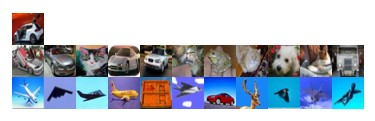
\includegraphics[width=\textwidth, height=5cm, natwidth=375, natheight=121]{deepinfodemo3.jpg}


\end{frame}


\subsection{Momentum Contrast}

\begin{frame}
	\frametitle{\insertsection}
	\framesubtitle{\insertsubsection}

	Результати тестування алгоритму Momentum Contrast, $\tau = 0,7$, learning rate = 0,2. Помилка $-$ 37,42 \%, чотири години тренування.
	
    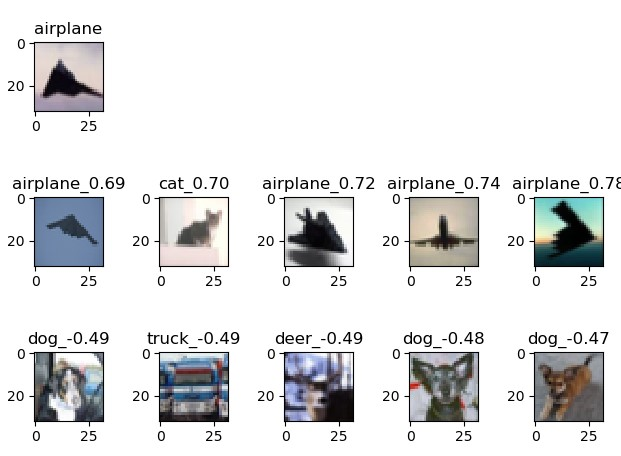
\includegraphics[width=\textwidth, height=8cm, natwidth=621, natheight=456]{mocodemo3.jpg}

\end{frame}

\section{Висновки}

\begin{frame}
	\frametitle{\insertsection}
	Виконання дипломної роботи складалося з наступних етапів:

	\begin{enumerate}
		\item проведення аналізу літературних джерел;\pause
		\item засвоєння алгоритмів Deep InfoMax та Momentum Contrast для вирішення задачі навчання без учителя;\pause
		\item реалізація методів Deep InfoMax та Momentum Contrast з використанням бібліотек мови програмування Python.
	\end{enumerate}

	Результати прогнозування показали, що алгоритм Deep InfoMax дає кращі результати, в той час як Momentum Constras $-$ більш вигідний з точки зору часу та обчислювальних ресурсів.
\end{frame}

\begin{frame}
	\centering\LARGEДякую за увагу!
\end{frame}

\end{document}
